\documentclass[conference]{IEEEtran}
\IEEEoverridecommandlockouts
\usepackage{cite}
\usepackage{amsmath,amssymb,amsfonts}
\usepackage{graphicx}
\usepackage{textcomp}
\usepackage{xcolor}
\usepackage{multirow}
\usepackage{array}
\usepackage{url}

\def\BibTeX{{\rm B\kern-.05em{\sc i\kern-.025em b}\kern-.08em
    T\kern-.1667em\lower.7ex\hbox{E}\kern-.125emX}}

\begin{document}

\title{An Automated PHP Legacy Code Migration Pipeline with Integrated
ISO/IEC 27001:2022 Security Compliance Analysis}

\makeatletter
\def\@IEEEauthorblockNstyle{\normalfont\normalsize}
\def\@IEEEauthorblockAstyle{\normalfont\normalsize}
\makeatother

\author{%
\IEEEauthorblockN{1\textsuperscript{st} Muhammad Farrel Akbar}
\IEEEauthorblockA{%
  \textit{Department of Electrical and}\\
  \textit{Information Engineering}\\
  \textit{Universitas Gadjah Mada}\\
  Yogyakarta, Indonesia\\
  muhammadfarrelakbar@mail.ugm.ac.id}
\and
\IEEEauthorblockN{2\textsuperscript{nd} Dani Adhipta}
\IEEEauthorblockA{%
  \textit{Department of Electrical and}\\
  \textit{Information Engineering}\\
  \textit{Universitas Gadjah Mada}\\
  Yogyakarta, Indonesia\\
  dani@ugm.ac.id}
\and
\IEEEauthorblockN{3\textsuperscript{rd} Ir.\ Addin Suwastono}
\IEEEauthorblockA{%
  \textit{Department of Electrical and}\\
  \textit{Information Engineering}\\
  \textit{Universitas Gadjah Mada}\\
  Yogyakarta, Indonesia\\
  adyn@ugm.ac.id}
}

\maketitle

\begin{abstract}
Most websites still run PHP applications on version 7.x or older
that no longer receive official security updates, leaving systems
exposed to an ever-growing accumulation of known vulnerabilities.
Manual migration across hundreds of source files is impractical,
and existing transformation tools do not incorporate security
compliance checks as an integrated part of the migration workflow.
Organizations operating under ISO/IEC 27001:2022 must also perform
security audits as a separate post-migration step, adding to the
operational burden. This research builds a Python-based pipeline
that integrates automatic conversion of legacy PHP web applications
to a configurable target PHP version with ISO/IEC 27001:2022
secure coding compliance checks in a single, fully local,
open-source workflow. The pipeline combines Rector for AST-based
code transformation, Semgrep for security scanning, PHPStan for
post-conversion type validation, and five open-source large
language models running locally via Ollama for semantic
vulnerability analysis and remediation suggestions. Case studies
were conducted on PHP codebases from FT UGM (245 files) and
CBT DTI UGM (326 files). Rector achieved conversion rates of
97.6\% and 91.7\% respectively, with 100\% post-conversion syntax
validity in both cases. A security finding delta of $\Delta F = 0$
confirmed that the conversion process introduced no new
vulnerabilities. Automatically generated JSON reports include
per-finding mappings to ISO/IEC 27001:2022 Annex A controls and
serve directly as audit documentation. Among five evaluated LLMs,
Qwen2.5-Coder 7b is recommended for pipeline integration,
consistently achieving a Syntax Validity Rate of 100\% across all
experimental conditions.
\end{abstract}

\begin{IEEEkeywords}
PHP migration, secure coding, ISO/IEC 27001:2022, large language
model, AST code transformation
\end{IEEEkeywords}

% ============================================================
\section{Introduction}
% ============================================================

PHP powers 71.7\% of all websites with a known server-side
language \cite{w3techs2024php}, yet nearly half of those sites
run versions that no longer receive official security updates:
33.1\% on PHP 7.x and 8.7\% on PHP 5.x \cite{w3techs2024php}.
Official support for PHP 7.4 ended on 28 November 2022
\cite{phpgroup2022supported}, leaving unpatched systems
permanently exposed to vulnerabilities catalogued by NIST NVD
\cite{nist_nvd}. Migrating to PHP 8.x is not a simple
search-and-replace operation: breaking changes---including the
removal of the entire \texttt{ext/mysql} extension, a stricter
type system, and altered error handling---affect large codebases
in ways that require structural analysis, not merely textual
substitution \cite{phpgroup2022supported}.

Available tools address parts of the problem in isolation.
Rector \cite{rector2024} handles AST-based syntactic
transformations reliably, as confirmed at production scale by
Chen et al.\ \cite{chen2022ast}, but cannot replace
\texttt{mysql\_*()} calls that require semantic understanding
of database access logic. Semgrep \cite{semgrep2024} and
PHPStan \cite{phpstan2024} detect security patterns and type
errors, but neither integrates into a migration workflow.
Crucially, none of these tools produces ISO/IEC 27001:2022
compliance evidence as a by-product of migration.

Organizations pursuing ISO/IEC 27001:2022 certification
\cite{iso27001_2022} must document adherence to Annex A.8.25
(secure development lifecycle), A.8.28 (secure coding), and
A.8.29 (security testing in development), requiring audit
evidence that code migration was conducted in accordance with
those controls---a burden currently met through manual work
entirely separate from the migration process.

Advances in locally deployable large language models
\cite{ollama2024} now make it feasible to provide semantic
analysis without transmitting source code to external services.
Li et al.\ \cite{li2025iris} showed that combining LLMs with
static analysis detects more vulnerabilities than either
approach alone. However, existing LLM-assisted approaches
\cite{akuthota2023vulnerability}\cite{stumpfle2025llm} use
cloud-based models and do not address version migration or
compliance standards.

This paper makes the following contributions: (1) a
Python-based pipeline that combines Rector, Semgrep, PHPStan,
and five locally running open-source LLMs into a single
automated workflow for PHP legacy code migration with integrated
ISO/IEC 27001:2022 compliance analysis; (2) empirical validation
on two real-world PHP codebases totaling 571 files; and (3) a
systematic comparison of five open-source LLMs on PHP security
remediation tasks, establishing Syntax Validity Rate (SVR) as
the most reliable evaluation metric for this context.

% ============================================================
\section{Related Work}
% ============================================================

\textbf{Automated PHP security remediation.}
Merlo et al.\ \cite{merlo2007automated} demonstrated in 2007
that automated static-and-dynamic analysis can protect legacy PHP
against SQL injection without altering functionality, achieving
zero false positives on phpBB 2.0.0. Their work confirms that
automated PHP security analysis is feasible; the gap is that no
comprehensive solution operating against modern security standards
has emerged in the intervening decades.

\textbf{LLM-based vulnerability detection.}
Akuthota et al.\ \cite{akuthota2023vulnerability} showed
that GPT-3.5-Turbo can identify common vulnerability patterns via
prompt engineering alone, with accuracy degrading as pattern
complexity increases. Li et al.\ \cite{li2025software} improved
results by combining patch history with structured static
analysis. Both studies use cloud APIs, creating a data privacy
barrier for institutions managing confidential source code.
Li, Dutta, and Naik \cite{li2025iris} introduced IRIS, which
combines LLMs with CodeQL for whole-repository taint analysis,
detecting 55 of 120 CWE-Bench-Java vulnerabilities versus 27
by CodeQL alone. IRIS relies on GPT-4 via the cloud and targets
Java; this work adopts a conceptually similar combined approach
but with local models targeting PHP.

\textbf{LLM-assisted code transformation.}
St\"{u}mpfle et al.\ \cite{stumpfle2025llm} used LLMs for
software variant migration into a Software Product Line,
employing a self-refinement loop that feeds compilation test
results back to the model iteratively. The feedback loop serves
a similar role to PHPStan post-conversion validation in this
pipeline. A fundamental difference is focus: their work targets
cross-variant feature extraction; this work targets PHP version
migration and security compliance.

\textbf{Long-term consequences of automated transformation.}
Strobl et al.\ \cite{strobl2020automated} analyzed three
government-sector automated COBOL/PL/I-to-Java conversions each
exceeding one million lines, finding that the absence of embedded
validation mechanisms caused problems that only emerged after
deployment. This finding motivates the inclusion of PHPStan and
dual Semgrep scans (pre- and post-conversion) in this pipeline.

\textbf{AST-based migration at industrial scale.}
Chen et al.\ \cite{chen2022ast} demonstrated that AST-based
symbol replacement can migrate large-scale TypeScript codebases
at Microsoft with negligible functional regression, validating
the reliability of the Rector-based approach adopted here.
Neither Cai et al.\ \cite{cai2015pattern} nor Chen et al.\
address security or standards compliance.

Taken together, no prior work combines PHP version migration,
locally running LLM security analysis, post-conversion static
validation, and ISO/IEC 27001:2022 compliance reporting in a
single open-source workflow.

% ============================================================
\section{System Architecture}
% ============================================================

\subsection{Pipeline Overview}

The pipeline consists of six Python modules orchestrated by
\texttt{main.py}. Modules execute sequentially; all inter-module
communication passes as in-memory Python objects. The modular
design allows any component to be replaced or improved
independently. Fig.~\ref{fig:architecture} shows the pipeline
architecture.

\begin{figure}[htbp]
  \centering
  
\includegraphics[width=0.9\columnwidth]{contents/chapter-3/arsitektur-sistem.png}
  \caption{Pipeline system architecture with six functional modules
  and one orchestrator (\texttt{main.py}).}
  \label{fig:architecture}
\end{figure}

\subsection{Module Descriptions}

\textbf{Scanner} (\texttt{scanner.py}) runs Semgrep with the
\texttt{p/php} and \texttt{p/owasp-top-ten} rulesets on the
\texttt{input/} directory before conversion (pre-scan), then again
on \texttt{output/} after conversion (post-scan). The difference
$\Delta F = F_{\text{post}} - F_{\text{pre}}$ measures whether
the conversion introduced or eliminated vulnerabilities. Findings
are classified by vulnerability type and mapped to ISO/IEC
27001:2022 controls via keyword matching on \texttt{rule\_id} and
\texttt{message} fields.

\textbf{Converter} (\texttt{converter.py}) copies all PHP files
from \texttt{input/} to \texttt{output/}, then runs Rector with
a runtime-generated configuration targeting the specified PHP
version. Rector applies a cumulative \texttt{LevelSetList} chain
from \texttt{UP\_TO\_PHP\_53} through the target version plus
\texttt{SetList::CODE\_QUALITY}, \texttt{DEAD\_CODE},
\texttt{EARLY\_RETURN}, and \texttt{TYPE\_DECLARATION} sets.
The \texttt{input/} directory is never modified; failed files
remain in \texttt{output/} as copies of the original.

\textbf{Analyzer} (\texttt{analyzer.py}) runs PHPStan level 5
on \texttt{output/} to verify type correctness and compatibility
with the target PHP version. Each finding is tagged with the
relevant ISO/IEC 27001:2022 control and classified as ERROR or
WARNING.

\textbf{AI Engine} (\texttt{ai\_engine.py}) receives Semgrep
pre-scan findings with priority levels 1--5 (SQL Injection, XSS,
deprecated functions, hardcoded credentials, path traversal /
SSRF) and sends each one to the selected LLM via the Ollama REST
API at \texttt{localhost:11434}. The prompt requests a
vulnerability explanation, a secure PHP 8.x replacement in a
fenced code block, and a \texttt{CONFIDENCE: [0-100]} line. Code
blocks are extracted by markdown pattern matching and validated
with \texttt{php -l}. The module is automatically skipped if no
findings exceed the priority threshold or if Ollama is
unavailable.

\textbf{ISO Mapper} (\texttt{iso\_mapper.py}) collects all
findings from the Scanner, Analyzer, and AI Engine as in-memory
objects and applies deterministic rule-based mapping to six
ISO/IEC 27001:2022 Annex A controls: A.5.17 (authentication
information), A.8.24 (use of cryptography), A.8.25 (secure
development lifecycle), A.8.26 (application security
requirements), A.8.28 (secure coding), and A.8.29 (security
testing in development). Rule-based mapping was chosen over
AI-based mapping to ensure deterministic, auditable results.
Per-control status is \texttt{COMPLIANT} (no findings),
\texttt{NON\_COMPLIANT} (active Semgrep findings), or
\texttt{PARTIAL} (PHPStan-only findings).

\textbf{Composer Analyzer} (\texttt{composer\_analyzer.py})
checks PHP 8.x compatibility of each dependency declared in
\texttt{composer.json} using Packagist metadata. The module is
automatically skipped if no \texttt{composer.json} is present.

\texttt{main.py} combines all module outputs into a structured
JSON report in \texttt{reports/} and displays a Rich-formatted
console summary. The JSON report is designed to serve directly
as ISO/IEC 27001:2022 audit documentation. The complete pipeline
source code is publicly available at
\url{https://github.com/MFarrelAkbar1/skripsi-php-migration}.

\subsection{LLM Evaluation Metrics}

Five metrics are applied. The \textbf{Rector Conversion Rate}
(CR) is $f_{\text{success}} / f_{\text{total}} \times 100\%$.
The \textbf{Format Compliance Rate} (FCR) adapts prompt-level
strict-accuracy from IFEval \cite{zhou2023ifeval}: a response is
compliant only if it contains all three required elements
simultaneously (explanation, PHP code block, and
\texttt{CONFIDENCE:} line). The \textbf{Syntax Validity Rate}
(SVR) adapts pass@1 \cite{roziere2024codellama}: the percentage
of extracted code blocks that pass \texttt{php -l}. SVR is
designated the primary metric because it is independently
verifiable. The \textbf{Security Finding Delta}
$\Delta F = F_{\text{post}} - F_{\text{pre}}$ measures the
post-conversion security posture change. The \textbf{Mean
Confidence Score} $\bar{C}_m$ is a secondary metric recording
the model's self-reported score; prior work confirms that
small-to-medium LLMs are poorly calibrated
\cite{akuthota2023vulnerability}\cite{li2025iris}.

% ============================================================
\section{Results and Discussion}
% ============================================================

\subsection{Datasets}

Case Study 1 uses 245 PHP files from the TCK Dashboard
application of FT UGM (Faculty of Engineering, Universitas
Gadjah Mada), built on CodeIgniter 3.x with PHP 7.4.9. Case
Study 2 uses 326 PHP files from the Computer-Based Test (CBT)
application of DTI UGM (Directorate of Information Technology),
built on CodeIgniter 3.x with a PHP $\geq$ 7.0 requirement.
Both codebases were used solely for static analysis in a local
environment; no source code was transmitted to any external
service.

\subsection{Rector Conversion Results}

Rector was run with a PHP 8.3 target on both datasets.
Fig.~\ref{fig:rector-comparison} compares conversion results
across both case studies.

\begin{figure}[htbp]
  \centering
  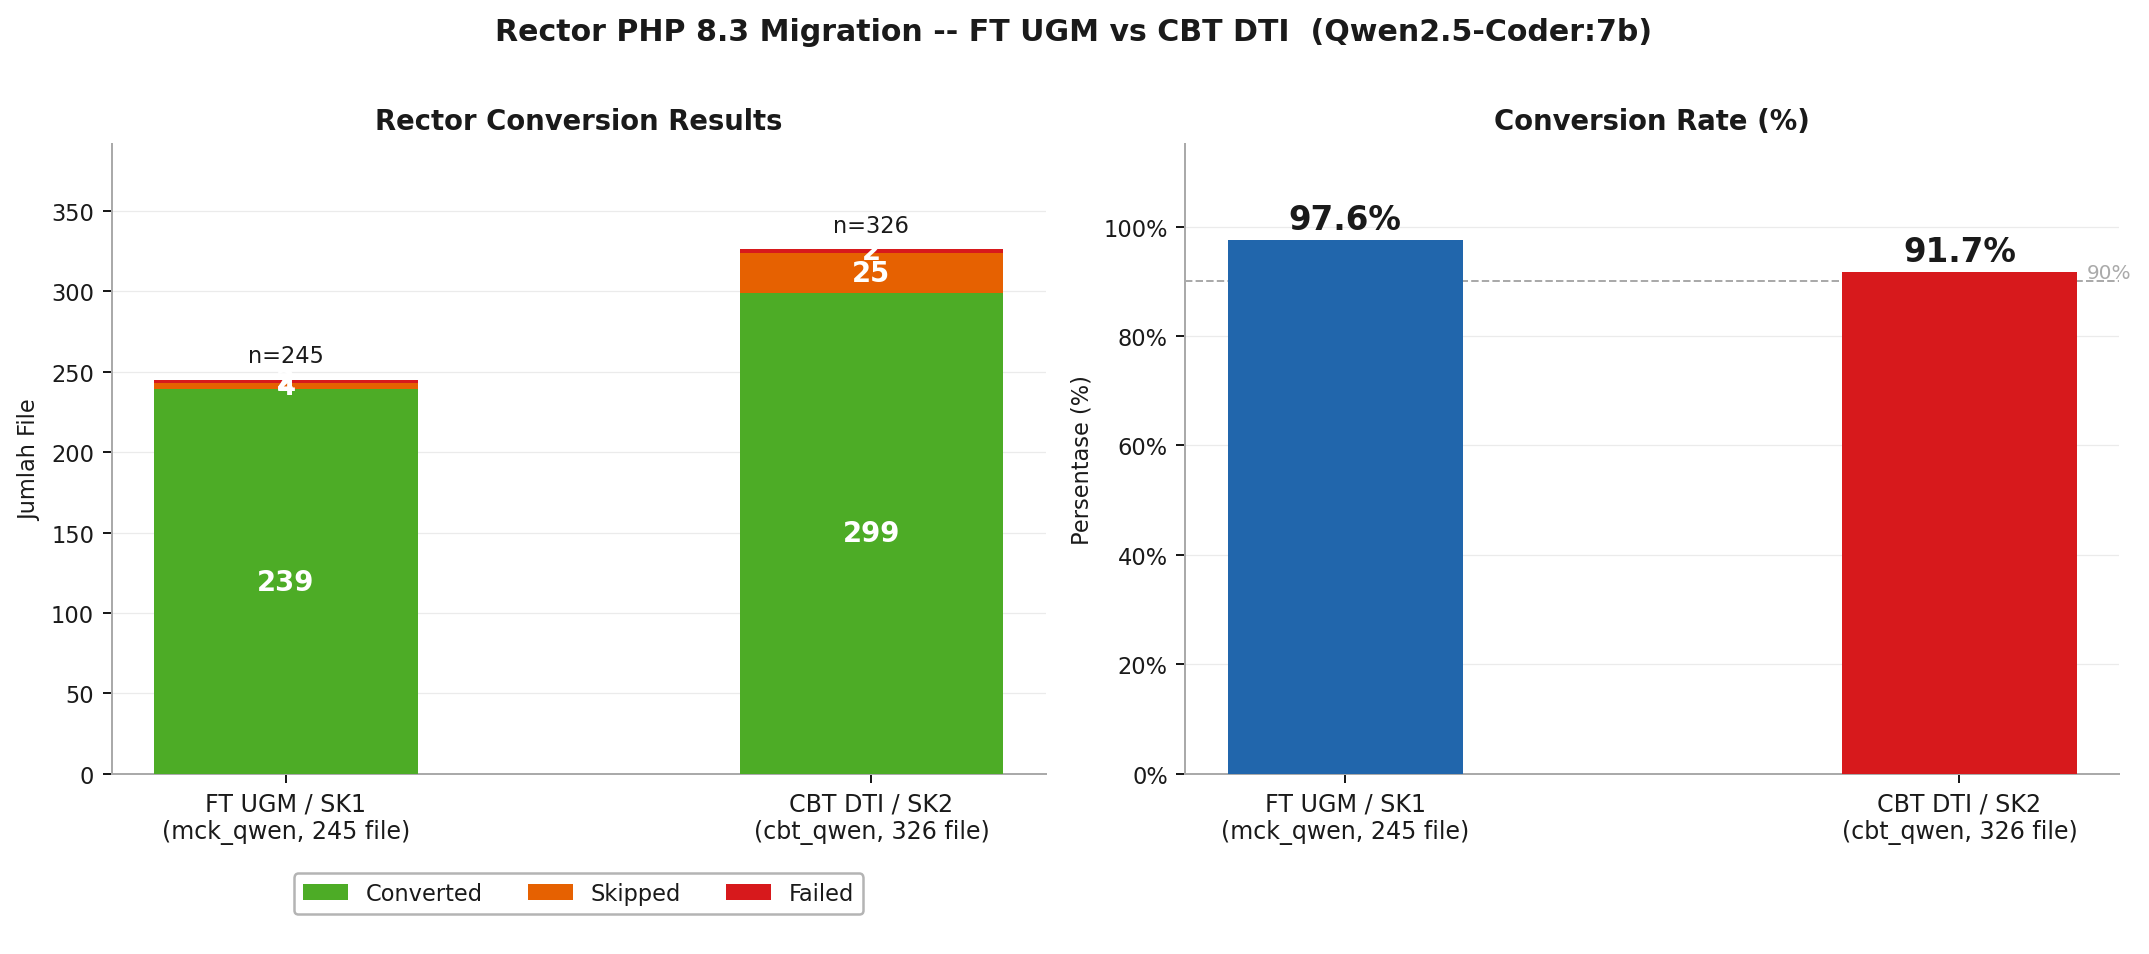
\includegraphics[width=\columnwidth]{contents/chapter-4/comparison/comparison_qwen_2_rector_conversion.png}
  \caption{Comparison of Rector conversion results for both case
  studies (FT UGM: 245 files; CBT DTI UGM: 326 files).}
  \label{fig:rector-comparison}
\end{figure}

FT UGM achieved a conversion rate of 97.6\% (239 converted,
4 skipped, 2 failed). CBT DTI achieved 91.7\% (299 converted,
25 skipped, 2 failed). The 5.9 percentage point difference is
primarily attributable to a higher proportion of skipped files
in CBT DTI (7.7\% vs.\ 1.6\%): skipped files already satisfy
PHP 8.3 requirements and do not require transformation.

In both datasets, exactly 2 files failed with the same internal
\texttt{FiberNodeScopeResolver} bug in the Rector version used,
triggered by branch patterns returning heterogeneous types
(\texttt{captcha\_helper.php}) or by large numbers of
\texttt{if (!function\_exists(\ldots))} constructs
(\texttt{form\_helper.php}). This failure is systemic to the
Rector version, not a property of the source code. All files
in \texttt{output/} passed \texttt{php -l} after conversion,
yielding a post-conversion syntax validity rate of 100\% for
both case studies.

Sampling-based accuracy validation on 24 randomly selected files
(10\% of valid files, fixed seed for reproducibility) found that
Rector output and an LLM-assisted
manual reference achieved identical syntax validity (100\%) and
deprecated removal rates (100\%), with a mean line-level
similarity score of 0.9214 (11 of 12 application-layer files
in the 0.90--1.00 range).

\subsection{Semgrep Security Scan Results}

Semgrep produced 11 findings in each dataset: 1 SQL Injection
and 10 SSRF, all concentrated in
\texttt{system/core/Output.php}, a core component of
CodeIgniter 3.x shared by both applications.
$\Delta F = 0$ in both case studies confirms that Rector's
AST-based transformation introduced no new vulnerabilities.
The pre-existing findings require remediation at the framework
code level, which lies outside the scope of syntactic
transformation.

\subsection{PHPStan Validation Results}

PHPStan level 5 targeting PHP 8.3 produced 2,790 findings for
FT UGM and 2,354 for CBT DTI. In both datasets, a substantial
fraction are false positives arising from PHPStan's inability to
trace CodeIgniter 3.x's dynamic architecture (magic properties
such as \texttt{\$this->db} and runtime-loaded helper functions
such as \texttt{base\_url()}): 354 and 318 items, respectively.
The remaining errors reflect technical debt---type
inconsistencies, undeclared return types, and missing dependency
classes---that existed prior to migration but were masked by PHP
7.x's permissive type system. The higher error count in FT UGM
despite its smaller file count is explained by the use of
third-party libraries (\texttt{PhpOffice\textbackslash
PhpSpreadsheet}, \texttt{Dotenv\textbackslash Dotenv}) whose
classes PHPStan cannot resolve without a full dependency
installation. These findings are consistent with Strobl et al.\
\cite{strobl2020automated}, who observed that automated
transformation exposes latent code quality issues that only
become apparent under stricter runtime environments.

\subsection{ISO/IEC 27001:2022 Compliance Status}

Table~\ref{tab:pipeline-metrics} summarizes the primary pipeline
metrics and ISO compliance status for both case studies.

\begin{table}[htbp]
  \caption{Pipeline Metrics and ISO/IEC 27001:2022 Compliance
  Status for Both Case Studies}
  \label{tab:pipeline-metrics}
  \centering
  \renewcommand{\arraystretch}{1.2}
  \begin{tabular}{|l|c|c|}
    \hline
    \textbf{Metric} & \textbf{FT UGM} & \textbf{CBT DTI} \\
    \hline\hline
    PHP files analyzed        & 245   & 326   \\
    \hline
    Rector CR                 & 97.6\% & 91.7\% \\
    \hline
    Post-conv.\ syntax validity & 100\%  & 100\%  \\
    \hline
    Semgrep findings (pre)    & 11    & 11    \\
    \hline
    \quad SQL Injection        & 1     & 1     \\
    \hline
    \quad SSRF                 & 10    & 10    \\
    \hline
    $\Delta F$                & 0     & 0     \\
    \hline
    PHPStan findings          & 2,790 & 2,354 \\
    \hline
    A.5.17 Auth.\ Info.\      & \texttt{COMPLIANT} & \texttt{COMPLIANT} \\
    \hline
    A.8.24 Cryptography       & \texttt{COMPLIANT} & \texttt{COMPLIANT} \\
    \hline
    A.8.25 Dev.\ Lifecycle    & \texttt{NON\_COMPL.} & \texttt{NON\_COMPL.} \\
    \hline
    A.8.26 App.\ Security     & \texttt{NON\_COMPL.} & \texttt{NON\_COMPL.} \\
    \hline
    A.8.28 Secure Coding      & \texttt{NON\_COMPL.} & \texttt{NON\_COMPL.} \\
    \hline
    A.8.29 Security Testing   & \texttt{NON\_COMPL.} & \texttt{NON\_COMPL.} \\
    \hline
    ISO overall status        & \texttt{NON\_COMPL.} & \texttt{NON\_COMPL.} \\
    \hline
  \end{tabular}
\end{table}

The NON\_COMPLIANT status accurately reflects the pre-remediation
security posture of legacy codebases, not a pipeline failure.
COMPLIANT status for A.5.17 and A.8.24 indicates that the
Semgrep ruleset produced no hardcoded credential or weak
cryptography findings in either dataset. The JSON reports
generated automatically on each pipeline execution are
structured for direct use as ISO/IEC 27001:2022 audit
documentation, providing per-finding mappings to Annex A
controls without additional manual work.

\subsection{LLM Comparison Experiment}

The comparison experiment used the 11 Semgrep pre-scan findings
from FT UGM as input, with 3 runs per finding per model
(33 trials per model, 165 total) at a temperature of 0.1. Condition A
applied an identical zero-shot prompt to all models. Condition B
applied a per-model optimized prompt based on failure patterns
observed in Condition A.

Fig.~\ref{fig:fcr-cond-a} shows the Format Compliance Rate for
Condition A. Fig.~\ref{fig:svr-cond-a} shows the Syntax
Validity Rate and code block extraction rate for Condition A.
Table~\ref{tab:llm-comparison} summarizes FCR and SVR across
both conditions for all five models.

\begin{figure}[htbp]
  \centering
  
\includegraphics[width=\columnwidth]{contents/chapter-4/llm_chart_20260425_212836_2_format_compliance.png}
  \caption{Format Compliance Rate (FCR) for all five LLM models
  in Condition A (zero-shot, identical prompt, $n=33$ per model).}
  \label{fig:fcr-cond-a}
\end{figure}

\begin{figure}[htbp]
  \centering
  
\includegraphics[width=\columnwidth]{contents/chapter-4/llm_quality_chart_20260425_122619.png}
  \caption{Syntax Validity Rate (SVR) and code block extraction
  rate for all five LLM models in Condition A.}
  \label{fig:svr-cond-a}
\end{figure}

\begin{table}[htbp]
  \caption{FCR and SVR Comparison: Condition A vs.\ Condition B
  for All Five LLM Models ($n=33$ per model per condition)}
  \label{tab:llm-comparison}
  \centering
  \renewcommand{\arraystretch}{1.2}
  \begin{tabular}{|l|c|c|c|c|}
    \hline
    \multirow{2}{*}{\textbf{Model}} &
      \multicolumn{2}{c|}{\textbf{FCR}} &
      \multicolumn{2}{c|}{\textbf{SVR}} \\
    \cline{2-5}
     & \textbf{Cond.\ A} & \textbf{Cond.\ B} &
       \textbf{Cond.\ A} & \textbf{Cond.\ B} \\
    \hline\hline
    DeepSeek Coder 6.7b & 15\%  & \textbf{61\%} & 100\% & 100\%\\
    \hline
    Qwen2.5-Coder 7b    & 0\%   & 0\%   & \textbf{100\%} & \textbf{100\%} \\
    \hline
    CodeLlama 7b        & 100\% & 100\% & 27.3\%         & 39.4\%         \\
    \hline
    Mistral 7b          & 6\%   & 0\%   & 0\%            & 0\%            \\
    \hline
    Llama 3.1 8b        & 0\%   & 3\%   & 100\% & 0\%           \\
    \hline
    \multicolumn{5}{l}{SVR measured on $\leq$3 extracted blocks; not statistically representative.}
  \end{tabular}
\end{table}

The results reveal a systematic trade-off between FCR and SVR.
CodeLlama achieved 100\% FCR in both conditions but its SVR
was only 27.3\% (Condition A) and 39.4\% (Condition B): the
model follows format instructions consistently but generates
syntactically invalid PHP code in the majority of cases.
Qualitative inspection shows that CodeLlama correctly identifies
vulnerabilities but produces code blocks that fail to close
properly, or reformats code without actually fixing the issue.

Qwen2.5-Coder achieved 0\% FCR (it ignores format instructions
entirely) yet produced 97--100\% extraction rates and 100\% SVR
in both conditions. Its remediation suggestions also demonstrate
deeper semantic understanding: for the SQL Injection finding in
\texttt{Output.php} at line 768, Qwen2.5-Coder recognized that
the flagged code constructs a cache path rather than an SQL
query, and correctly applied \texttt{urlencode()} to the
\texttt{\$\_SERVER['QUERY\_STRING']} input.

Prompt optimization in Condition B produced significant
improvement only for models with sufficient baseline
instruction-following capability. DeepSeek Coder improved from
15\% to 61\% FCR when given shorter, more direct instructions,
confirming it was burdened by prompt complexity rather than
lacking capability. The few-shot strategy applied to Mistral
had the opposite effect (FCR dropped from 6\% to 0\%),
consistent with findings in the literature that prompt
engineering techniques effective for large models cannot always
be transferred to small-to-medium models \cite{akuthota2023vulnerability}.
CodeLlama's SVR limitation proved structural: its PHP 8.x code
generation quality did not materially improve despite explicit
syntax validation instructions.

Parameter sensitivity experiments (Condition C) on
Qwen2.5-Coder confirmed that its SVR is stable at 100\% across
temperatures 0.1--0.7. Increasing the context window from 2,000
to 4,000 characters raised the extraction rate from 97\% to
100\%, suggesting a marginal benefit for longer source files.

The mean confidence score $\bar{C}_m$ showed no reliable
correlation with code quality in any condition.
CodeLlama reported $\bar{C}_m = 0.909$ while producing
primarily invalid code; Qwen2.5-Coder reported
$\bar{C}_m = 0.000$ (no parseable confidence line) while
achieving 100\% SVR. This confirms that SVR---not FCR or
$\bar{C}_m$---is the most valid evaluation metric for locally
running LLM-based PHP security analysis systems, consistent
with calibration findings in \cite{akuthota2023vulnerability}
and \cite{yan2025codeif}.

\subsection{AI Engine Effectiveness Validation}

A blind rating experiment validated whether the AI Engine adds
measurable value over the raw pipeline output. Two output conditions
were compared: \textbf{B0}---pipeline output \emph{without} AI
Engine, containing only the Semgrep \texttt{rule\_id}, file name,
line number, severity, code snippet, and deterministic ISO control
mapping; and \textbf{T1}---pipeline output \emph{with} AI Engine
active using Qwen2.5-Coder 7b, which appends a natural-language
vulnerability explanation and a PHP 8.x remediation code suggestion
to each finding.

Two independent raters from DTETI FT UGM---unfamiliar with the
pipeline internals---assessed all 11 FT UGM Semgrep findings
(FT-01 to FT-11) presented as anonymous package pairs. B0/T1
assignment to Package A or B was randomized with a fixed seed
(\texttt{seed=42}). Each package was scored on four Likert-7
dimensions: Accuracy, Clarity, Actionability, and ISO mapping
correctness.

Table~\ref{tab:blind-rating} summarizes mean scores per dimension
(averaged over both raters). T1 outperformed B0 most strongly on
Clarity ($+0.591$ points) and Actionability ($+0.500$ points). No
meaningful difference appeared on Accuracy ($+0.045$) or ISO mapping
correctness ($0.000$), confirming that the deterministic rule-based
ISO Mapper already produces correct and sufficient control mappings
without LLM augmentation.

\begin{table}[htbp]
  \caption{Mean Scores per Dimension: B0 (Without AI Engine) vs.\
  T1 (With AI Engine), Likert-7 Scale, 2 Raters, $n = 11$ Findings}
  \label{tab:blind-rating}
  \centering
  \renewcommand{\arraystretch}{1.2}
  \begin{tabular}{|l|c|c|c|}
    \hline
    \textbf{Dimension} & \textbf{B0} & \textbf{T1} &
      \textbf{T1$-$B0} \\
    \hline\hline
    Accuracy        & 6.000 & 6.045 & $+$0.045 \\
    \hline
    Clarity         & 5.909 & 6.500 & $+$0.591 \\
    \hline
    Actionability   & 5.955 & 6.455 & $+$0.500 \\
    \hline
    ISO mapping     & 6.500 & 6.500 & \phantom{$+$}0.000 \\
    \hline
    \textbf{Overall}& \textbf{6.091} & \textbf{6.375} &
      $\mathbf{+0.284}$ \\
    \hline
  \end{tabular}
\end{table}

A one-sided Wilcoxon signed-rank test \cite{wilcoxon1945individual}
applied to the 10 SSRF findings (FT-02 to FT-11; the single SQL
Injection finding FT-01 was analyzed descriptively due to $n = 1$)
yielded $W = 44.0$, $p = 0.047$, confirming that T1 scores are
statistically significantly higher than B0 at $\alpha = 0.05$.
Inter-rater agreement measured by Cohen's kappa
\cite{cohen1960coefficient} was $\kappa = -0.097$ (poor), as Rater 1
assigned identical scores to both conditions for all findings while
Rater 2 showed position-dependent variation. Results on Clarity and
Actionability should therefore be interpreted with caution;
replication with a larger rater panel and a more diverse vulnerability
dataset is needed to strengthen statistical power.

% ============================================================
\section{Conclusions}
% ============================================================

This paper presented a Python-based pipeline that unifies
automated PHP legacy code migration, security scanning, and
ISO/IEC 27001:2022 compliance reporting into a single
open-source, fully local workflow. Four main conclusions follow.

First, Rector-based AST transformation achieved conversion rates
of 97.6\% and 91.7\% across two real-world CodeIgniter 3.x
codebases with 100\% post-conversion syntax validity in both
cases. The two failures per dataset were caused by a
reproducible Rector bug, not source code characteristics,
confirming the reliability of the approach for institutional
codebases.

Second, $\Delta F = 0$ in both case studies demonstrates that
automated AST-based transformation does not introduce new
security vulnerabilities---an important guarantee for
organizations whose operational continuity depends on the
integrity of migrated code. Automatically generated JSON
reports with per-finding ISO/IEC 27001:2022 control mappings
serve directly as audit documentation, eliminating the separate
manual compliance step currently required by organizations
pursuing certification.

Third, PHPStan validation exposed thousands of type
compatibility issues that PHP 7.x's permissive type system
had concealed, providing concrete pre-deployment evidence of
technical debt consistent with the findings of Strobl et al.\
\cite{strobl2020automated}.

Fourth, the AI Engine provides measurable added value over the
raw pipeline output. A blind rating experiment showed that T1
(with AI Engine) outperformed B0 (without AI Engine) on Clarity
($+0.591$ points) and Actionability ($+0.500$ points) on a Likert-7
scale; the overall difference of $+0.284$ points was confirmed
statistically significant by a one-sided Wilcoxon signed-rank test
($W = 44.0$, $p = 0.047$, $n = 10$). No difference was observed on
ISO mapping correctness, confirming that the deterministic ISO Mapper
does not require LLM augmentation. Among five evaluated LLMs,
Qwen2.5-Coder 7b is recommended for pipeline integration: it achieved
SVR = 100\% in every experimental condition and produced the most
semantically accurate remediation suggestions. FCR and SVR proved to
be independent, uncorrelated dimensions; SVR is the more practically
meaningful metric for automated code quality assessment.

Future work should strengthen LLM evaluation with automated semantic
test suites, replicate the AI Engine blind rating with a larger rater
panel and a more diverse vulnerability dataset, develop
CodeIgniter 3.x stubs to reduce PHPStan false positives, and extend
the pipeline to support CI/CD integration and additional programming
languages.

% ============================================================
\section*{Acknowledgment}
% ============================================================

The authors thank FT UGM and DTI UGM for providing access to
their PHP application source code for static analysis. All
analysis was conducted locally; no source code was transmitted
to external services.

\bibliography{references}{}
\bibliographystyle{IEEEtran}

\end{document}
